\chapter{The Lifetime of Objects}

Every object created by your application lives for an interval of time from its
creation to the point that the Java runtime gets around to collecting it. For
some subset of an object's {\em actual} lifetime, your application will make use
of its fields. An object's {\em natural} lifetime is defined by the interval of
time between its first and last necessary use. %%%%% cite drag paper here? It is
important to understand this distinction, between natural and actual lifetime, so
that you can implement your code in a way that avoids bugs and performs well in
the case when not everything fits into the Java heap.

The Java runtime helps manage some aspects of these management tasks, but leaves
a great deal of the work in your hands. In Java, you needn't explicitly free
objects, and in that way a managed language is a big step up from a language like
C. However, the promise of automatic memory management, that it frees you from
the burden of managing memory, doesn't play out as well in practice. Unless you
are careful, your program will suffer from bugs such as memory leaks, and suffer
from poor performance. Sometimes, your objects don't easily fit into the limits
of a single Java process, and you need to manage, explicitly, shuttling
them in and out of the Java heap.

When programming in Java it is important to think through whether your
application needs an object to live forever, or, if not, when you expect it to
die. With these thoughts in mind, you can plan how to  implement the right
lifetime policies. This entails combining the tools that Java  provides with
other strategies, implemented on top of Java.

\section{Common Categories of Natural Lifetime}

\begin{figure}
	\centering
	\subfigure[The lifecycle of a typical object and its data.]{
		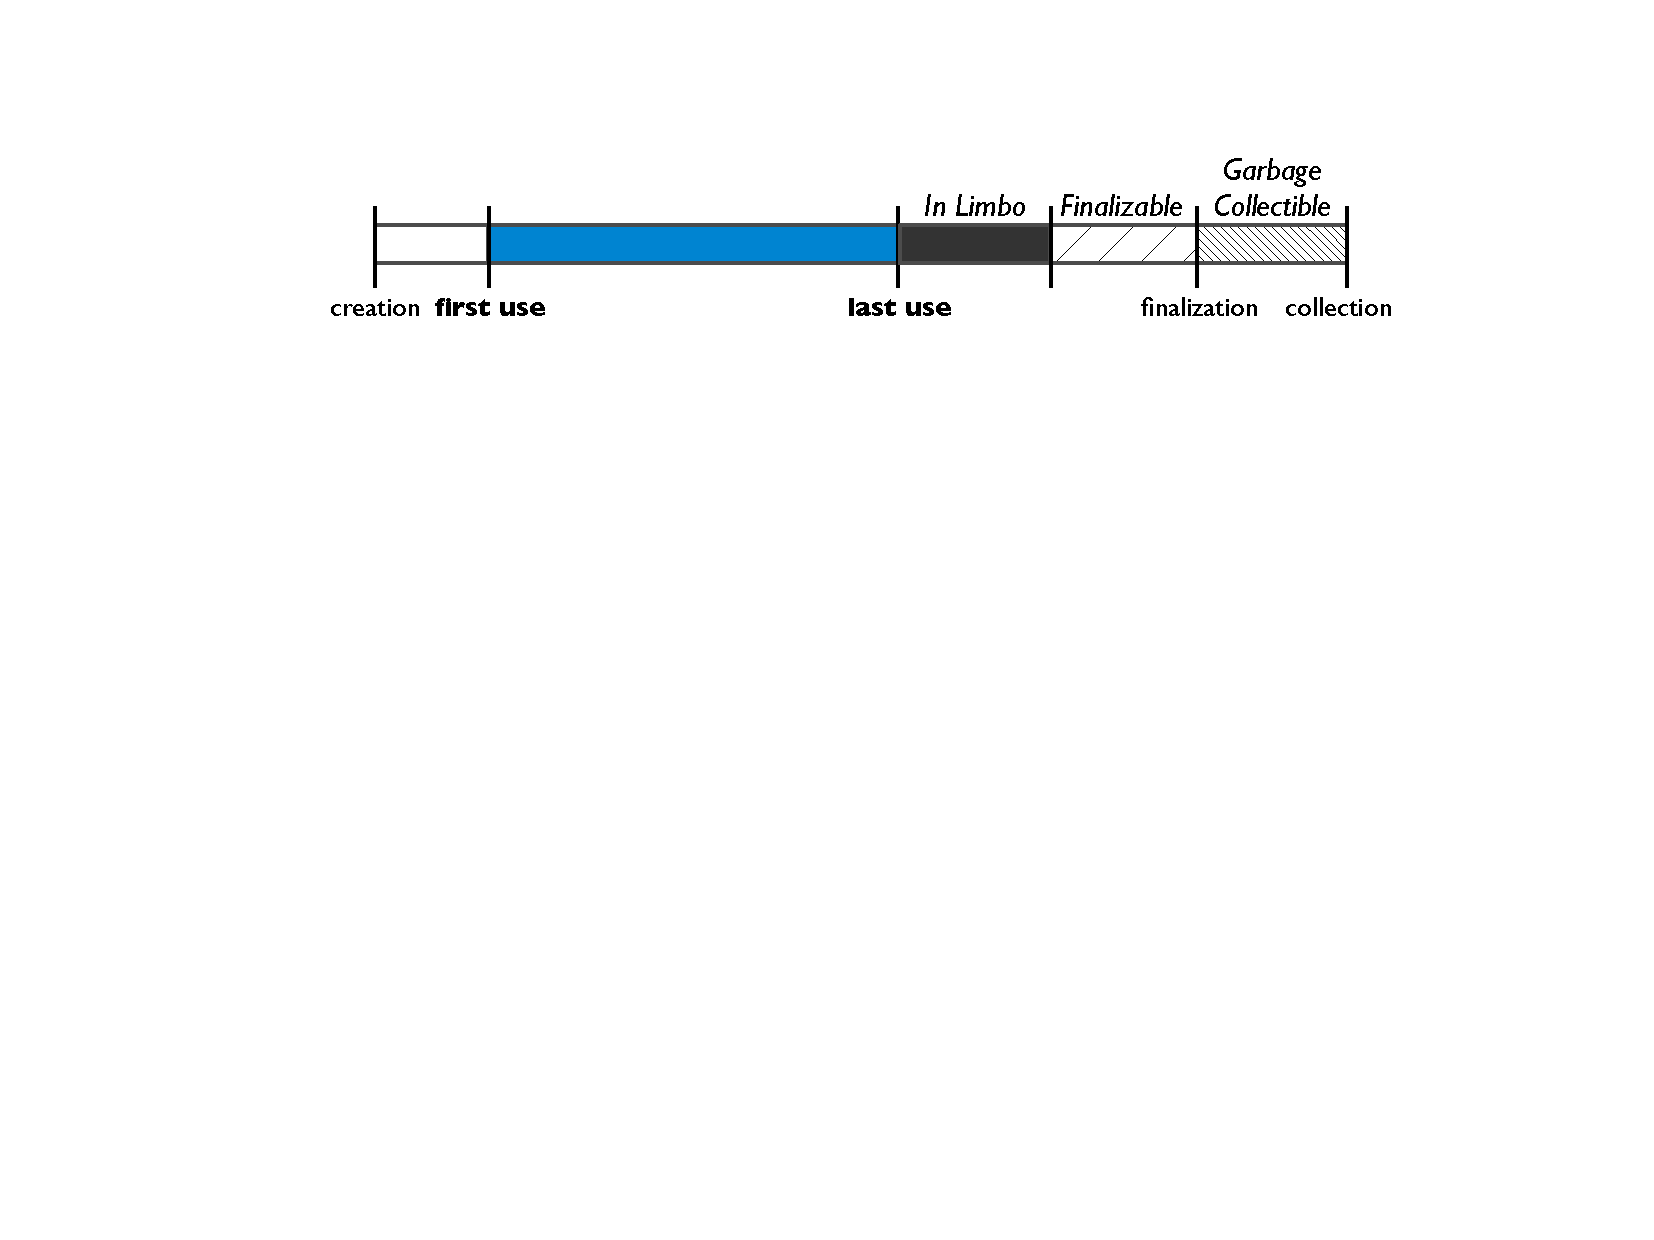
\includegraphics[width=0.9\textwidth]{Figures/object-lifecycle}
	}
	\subfigure[The lifecycle of the data  that is loaded from
	disk three times, and the objects that store it.]{
		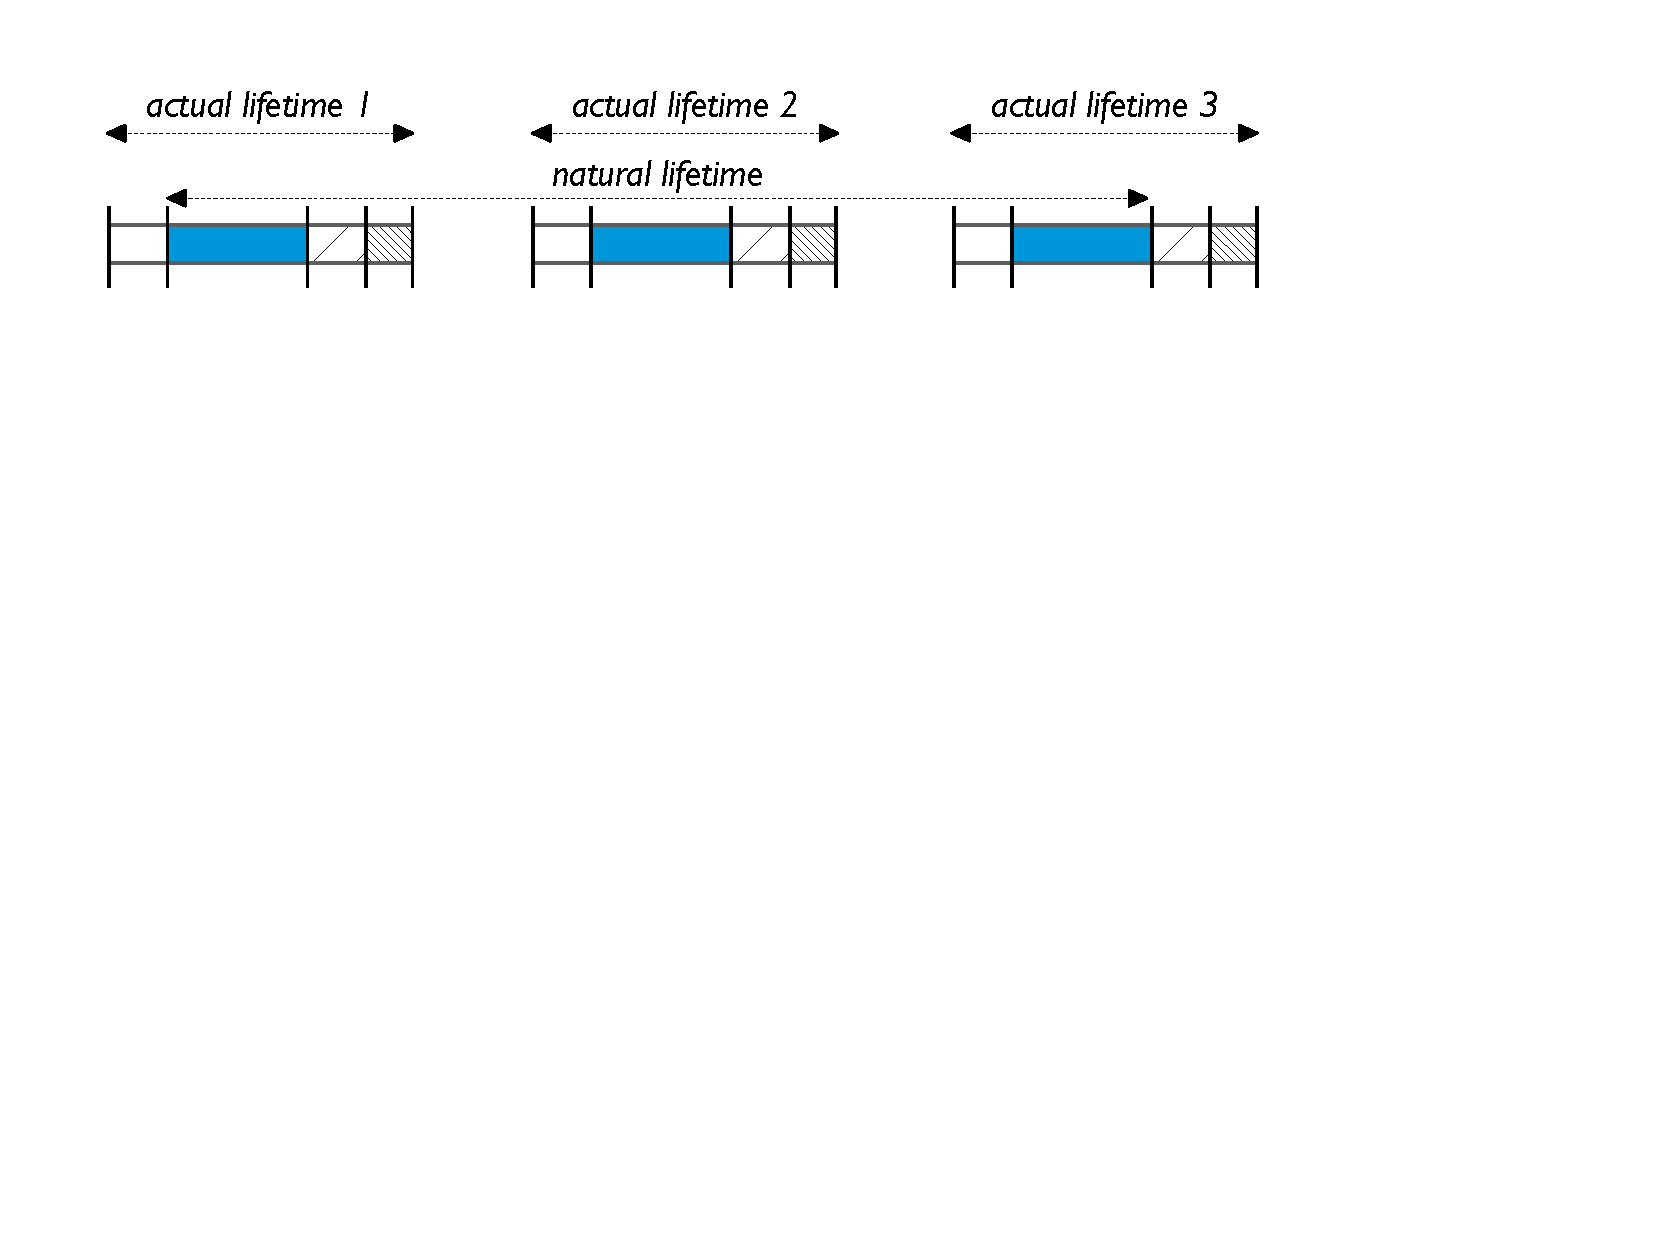
\includegraphics[width=0.9\textwidth]{Figures/object-lifecycle2}
	}
	\caption{Examples of Natural and Actual lifetimes.}
	\label{fig:typical-lifecycle}
\end{figure}


\begin{table}
\centering
	\begin{tabular}{lp{0.3\textwidth}p{0.35\textwidth}}
	\toprule  & Lifetime Property & Example \\ \midrule
	\autoref{temporary-lifetime}  & {Temporary} & new
	\class{SimpleDateFormat} to parse every date
	\\
	\autoref{forever-lifetime} & {Needed Forever} & product catalog
	\\
	\autoref{correlated-lifetime-1} & {Need Correlated with Another Object}
	& object annotations
	\\
	\autoref{correlated-lifetime-2} & {Need Correlated with Phase} &
	abstract syntaxt tree used only during parsing
	\\
	\autoref{deferred-deletion} & {Not Needed Now, but Deferred Deletion} &
	session state \\
%period\\ scoped to a phase/request\\
%correlated with an object (annotations)\\
%correlated with need}\\ \hline
%reusable & maybe i'll need it later \\ \hline
	\bottomrule
	\end{tabular}
	\caption{Five important categories of object lifetime.}
	\label{tab:five-lifetimes}
\end{table}

\autoref{tab:five-lifetimes} summarizes five important cases of object lifetime.
% introduced by example in this chapter, and
Many objects are either temporaries or needed for
the entire run of your application. Sometimes you create objects whose lifetime
is correlated with other objects or that should go away when a method invocation
completes. Sometimes you need to manage objects hanging around longer than their
current need, to avoid future recomputations or refetching of data in the case
when it is needed in the near future. 


\begin{table}
\centering
	\begin{tabular}{ll} \toprule
    	& Things Java Doesn't Do Automatically \\ \midrule
    	\autoref{avoiding-lifetime-bugs} & {Avoiding Memory Leaks} \\
    	\autoref{balance-time-and-space} & {Balancing Time and Space} \\
    	\autoref{outisde-java-box} & {Supporting Massive Data Sets}  	\\
        \bottomrule
    \end{tabular}
	\caption{}
	\label{}
\end{table}


\section{Temporary Objects}
\label{temporary-lifetime}

If your application is like every other Java application ever written, it creates
a large number of temporary objects. Temporary objects are those that you create
to glue code together. They help to bridge one protocol with another. They enable
code reuse: as long as you can convert your data layout into a form that an API
requires, then you can reuse the functionality it provide. A great many of these
structures serve the role of a kind of lubricant, making it easy for you to write
code that ties together the separately written parts of your code base and reuses
standard libraries as much as possible. These are objects that are not a
fundamental necessity of what you're trying to accomplish, but a necessary
penalty one must pay when developing in the large.

A common example of this is the sequence of operations performed to parse and
manipulate data coming and going to the outside world. 
% to the wire?

\begin{example}{Temporary Objects}

Consider the code in \autoref{TempExampleCode}. This code starts in
the \code{main} method by splitting the input string into two substrings. So
far, the code has created four objects (one \class{String} and one character
array per substring). 
Creating these substrings makes it easy to use the \code{doWork} method, which
takes two Strings as input. However, observe
that these four objects are not a necessary part of the computation. Indeed,
these substrings are eventually used only as input to the
\class{SimpleDateFormat} \code{parse} method, which has been nicely designed to
allow you to avoid this very problem. By passing a \class{ParsePosition}, one
can parse substrings of a string without having to create temporary strings (at
the expense of creating temporary \class{ParsePosition} objects!).



\begin{lstlisting}[float,caption=An example that constructs 8 temporary
objects to handle two dates.,label=TempExampleCode]
void main(String xy) {
	doWork(xy.substring(0,10), xy.substring(10));
}
	
void doWork(String x, String y) {
	doRemoveProcedureCall(parse(x));
	doRemoveProcedureCall(parse(y));
}
	
Date parse(String string) {
	return new SimpleDataFormat().parse(string, new ParsePosition(0));
}

void doRemoteProcedureCall(Date date) {
	long timestamp = date.getTime();
	...
}
\end{lstlisting}

\end{example}

% correlated with need: as soon as last user goes away, remove his stuff 
% share common expressions to save space, but using strong references -> memory
% leak; plugins in eclipse go away when all views
% sharing pool 

% weak ref keys -> annotation
% weak ref values -> sharing pool

% soft ref values -> caching

% annotation by map lookup


\section{Objects Needed Forever}
\label{forever-lifetime}

Created and used for the remaining duration of a run.


\section{Objects with Correlated Lifetimes}

Many objects are created and then only needed for some interval of time. For
example, say your application is a transaction processing system implemented as
a Java Enterprise Edition web application. In this case, most objects
created within the scope of a servlet request will not, and for correctness
reasons {\em must not}, survive the request; they are not used by the 
application after the request has completed, and will, in the absence of bugs,
be collected as soon as is convenient for the runtime. In this example, the
lifetime of objects during a request are {\em correlated} with a method
invocation: when the servlet \class{doGet} or \class{doPut} (etc.) invocations
return, those correlated objects had better be garbage collectible.

The same is true for a great many objects created by the application, not just
at the large granularity of a servlets. For example,

In many cases, the built-in mechanisms 

\subsection{Correlated with Another Object}
\label{correlated-lifetime-1}

\subsection{Correlated with Need}
\label{correlated-lifetime-2}

\section{Objects with Deferred-Deletion}
\label{deferred-deletion}

A cache is a performance optimization that holds on to a data structure after the
current operation is finished with it, in the hope that other operations in the
near future will reuse it. The expense of re-fetching data from external data
sources and recomputing the in-memory structure can often be amortized, at the
expense of stretching the lifetime of these data structures. By increasing the
actual lifetime on an object you will very likely increase peak memory
consumption.




%if scopes don't coincide with lifetime

\begin{table}
\centering
\begin{tabular}{|l|l|} \hline
\em mechanism & \\ \hline \hline
stack & \\ \hline 
static & \\ \hline
thread-local & \\ \hline
soft & \\ \hline
weak & \\ \hline
phantom/finalizers & \\ \hline
memory mapping & via \texttt{java.nio} \\ \hline 
object serialization & \\ \hline
\end{tabular}
\caption{Built-in lifetime management mechanisms.}
\label{tab:builtin-lifetime-management}
\end{table}

\begin{table}
\centering
\begin{tabular}{|l|l|} \hline
\em mechanism & \\ \hline \hline
resource pool & \\ \hline
cache & \\ \hline
sharing pool & (interning)\\ \hline
memoization & \\ \hline
backing store &(externalized memo) \\ \hline
non-OO & (column orientation) \\ \hline 
\end{tabular}
\caption{Lifetime management mechanisms not provided by the Java language that one must implement.}
\label{tab:software-lifetime-management}
\end{table}




%% OLD STUFF NMM 20090820
%\section{Request Scoping}
%\section{Correlated Lifetime}
%\paragraph{Weak and Soft references in Java}
%\section{Memory Leaks and Drag}
%\section{Examples}
%\subsection{Transient Near-Copies}
%\subsubsection{String Canonicalization}
%\subsection{Temporary Collections}
%\subsection{Facilitators}
